\section{File Import/Export}
The commands \cmdlink{readFile} and \cmdlink{putsFile} simplify file I/O in Tcl. 
\begin{syntax}
\command{readFile} <\$option \$value ...> <-newline> \$file
\end{syntax}
\begin{args}
\$option \$value ... & File configuration options, see Tcl \textit{fconfigure} command. \\
-newline & Option to read the final newline if it exists. \\
\$file & File to read data from.
\end{args}
\begin{syntax}
\command{putsFile} <\$option \$value ...> <-nonewline> \$file \$string
\end{syntax}
\begin{args}
\$option \$value ... & File configuration options, see Tcl \textit{fconfigure} command. \\
-nonewline & Option to not write a final newline. \\
\$file & File to write data to. \\
\$string & Data to write to file.
\end{args}
\begin{example}{File import/export}
\begin{lstlisting}
# Export data to file (creates or overwrites the file)
putsFile example.txt "hello world"
# Import the contents of the file (requires that the file exists)
puts [readFile example.txt]
\end{lstlisting}
\tcblower
\begin{lstlisting}
hello world
\end{lstlisting}
\end{example}

\clearpage
\section{Data Conversion}
This package also provides conversion utilities for different datatypes. 
The main datatype is matrix, or \textbf{mat}. 
\subsection{Matrix (mat)}
The matrix (\textbf{mat}) datatype is a nested Tcl list, where each list element represents a row vector of equal length.
This definition is compatible with the matrix data type provided by the \textcolor{blue}{\href{https://github.com/ambaker1/ndlist}{ndlist}} package. 

An example of a matrix with headers is shown below. 
\begin{example}{Example data (\textbf{mat}):}
\begin{lstlisting}
set mat {{step disp force} {1 0.02 4.5} {2 0.03 4.8} {3 0.07 12.6}}
\end{lstlisting}
\end{example}
This format can be converted from and to all other formats, as is illustrated in the diagram below, with ``\textbf{a}'' and ``\textbf{b}'' acting as placeholders for all other datatypes.
\begin{center}
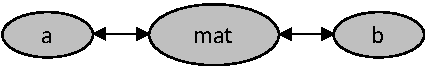
\includegraphics{figures/dataconversion.pdf}
\end{center}
This way, each new datatype only requires the addition of two new conversion commands: one to \textbf{mat} and one from \textbf{mat}.
Then, you can convert between any datatype using \textbf{mat} as the intermediate datatype.
\clearpage
\subsection{Table (tbl)}
The table (\textbf{tbl}) datatype is a key-value paired list, with keys representing the table header, and values representing the columns.
This definition is compatible with the table data type provided by the \textcolor{blue}{\href{https://github.com/ambaker1/taboo}{taboo}} package.
To convert between \textbf{mat} and \textbf{tbl}, use the commands \cmdlink{mat2tbl} and \cmdlink{tbl2mat}.
\begin{syntax}
\command{mat2tbl} \$mat
\end{syntax}
\begin{syntax}
\command{tbl2mat} \$tbl
\end{syntax}
\begin{args}
\$mat & Matrix value. \\
\$tbl & Table value. 
\end{args}
\begin{example}{Example data (\textbf{tbl}):}
\begin{lstlisting}
puts [mat2tbl $mat]
\end{lstlisting}
\tcblower
\begin{lstlisting}
step {1 2 3} disp {0.02 0.03 0.07} force {4.5 4.8 12.6}
\end{lstlisting}
\end{example}
\clearpage
\subsection{Space-Delimited Text (txt)}
The space-delimited text (\textbf{txt}) datatype is simply space-delimited values, where new lines separate rows. 
Escaping of spaces and newlines is consistent with Tcl rules for valid lists. 
To convert between \textbf{mat} and \textbf{txt}, use the commands \cmdlink{mat2txt} and \cmdlink{txt2mat}. 
\begin{syntax}
\command{mat2txt} \$mat 
\end{syntax}
\begin{syntax}
\command{txt2mat} \$txt
\end{syntax}
\begin{args}
\$mat & Matrix value. \\
\$txt & Space-delimited values.
\end{args}
\begin{example}{Example data (\textbf{txt}):}
\begin{lstlisting}
puts [mat2txt $mat]
\end{lstlisting}
\tcblower
\begin{lstlisting}
step disp force
1 0.02 4.5
2 0.03 4.8
3 0.07 12.6
\end{lstlisting}
\end{example}
\clearpage
\subsection{Comma-Separated Values (csv)}
The comma-separated values (\textbf{csv}) datatype is comma delimited values, where new lines separate rows. 
Commas and newlines are escaped with quotes, and quotes are escaped with double-quotes. 
To convert between \textbf{mat} and \textbf{csv}, use the commands \cmdlink{mat2csv} and \cmdlink{csv2mat}. 
\begin{syntax}
\command{mat2csv} \$mat
\end{syntax}
\begin{syntax}
\command{csv2mat} \$csv
\end{syntax}
\begin{args}
\$mat & Matrix value. \\
\$csv & Comma-separated values.
\end{args}
\begin{example}{Example data (\textbf{csv}):}
\begin{lstlisting}
puts [mat2csv $mat]
\end{lstlisting}
\tcblower
\begin{lstlisting}
step,disp,force
1,0.02,4.5
2 0.03,4.8
3,0.07,12.6
\end{lstlisting}
\end{example}
\clearpage
\subsection{Derived Conversions}
Using the \textbf{mat} datatype as the intermediate datatype, data can be converted to and from any datatype. 
As a convenience, shortcuts are provided for conversions that use \textbf{mat} as an intermediate data format.
\begin{syntax}
\command{tbl2txt} \$tbl \\
\command{tbl2csv} \$tbl
\end{syntax}
\begin{syntax}
\command{txt2tbl} \$txt \\
\command{txt2csv} \$txt
\end{syntax}
\begin{syntax}
\command{csv2tbl} \$csv \\
\command{csv2txt} \$csv
\end{syntax}
\begin{args}
\$tbl & Table value. \\
\$txt & Space-delimited values. \\
\$csv & Comma-separated values.
\end{args}
\begin{example}{Combining data conversions}
\begin{lstlisting}
# Convert from table to csv, using mat as an intermediate datatype.
set tbl {step {1 2 3} disp {0.02 0.03 0.07} force {4.5 4.8 12.6}}
set csv [mat2csv [tbl2mat $tbl]]; # also could use tbl2csv
puts $csv
\end{lstlisting}
\tcblower
\begin{lstlisting}
step,disp,force
1,0.02,4.5
2,0.03,4.8
3,0.07,12.6
\end{lstlisting}
\end{example}
\clearpage